%%%%%%%%%%%%%%%%%%%%%%%%%%%%%%%%%%%%%%%%%
% Beamer Presentation
% LaTeX Template
% Version 1.0 (10/11/12)
%
% This template has been downloaded from:
% http://www.LaTeXTemplates.com
%
% License:
% CC BY-NC-SA 3.0 (http://creativecommons.org/licenses/by-nc-sa/3.0/)
%
%%%%%%%%%%%%%%%%%%%%%%%%%%%%%%%%%%%%%%%%%

%----------------------------------------------------------------------------------------
%	PACKAGES AND THEMES
%----------------------------------------------------------------------------------------

\documentclass{beamer}

\mode<presentation> {

% The Beamer class comes with a number of default slide themes
% which change the colors and layouts of slides. Below this is a list
% of all the themes, uncomment each in turn to see what they look like.

%\usetheme{default}
%\usetheme{AnnArbor}
\usetheme{Antibes}
%\usetheme{Bergen}
%\usetheme{Berkeley}
%\usetheme{Berlin}
%\usetheme{Boadilla}
%\usetheme{CambridgeUS}
%\usetheme{Copenhagen}
%\usetheme{Darmstadt}
%\usetheme{Dresden}
%\usetheme{Frankfurt}
%\usetheme{Goettingen}
%\usetheme{Hannover}
%\usetheme{Ilmenau}
%\usetheme{JuanLesPins}
%\usetheme{Luebeck}
%\usetheme{Madrid}
%\usetheme{Malmoe}
%\usetheme{Marburg}
%\usetheme{Montpellier}
%\usetheme{PaloAlto}
%\usetheme{Pittsburgh}
%\usetheme{Rochester}
%\usetheme{Singapore}
%\usetheme{Szeged}
%\usetheme{Warsaw}

% As well as themes, the Beamer class has a number of color themes
% for any slide theme. Uncomment each of these in turn to see how it
% changes the colors of your current slide theme.

%\usecolortheme{albatross}
%\usecolortheme{beaver}
%\usecolortheme{beetle}
%\usecolortheme{crane}
%\usecolortheme{dolphin}
%\usecolortheme{dove}
\usecolortheme{fly}
%\usecolortheme{lily}
%\usecolortheme{orchid}
%\usecolortheme{rose}
%\usecolortheme{seagull}
%\usecolortheme{seahorse}
%\usecolortheme{whale}
%\usecolortheme{wolverine}

%\setbeamertemplate{footline} % To remove the footer line in all slides uncomment this line
%\setbeamertemplate{footline}[page number] % To replace the footer line in all slides with a simple slide count uncomment this line

%\setbeamertemplate{navigation symbols}{} % To remove the navigation symbols from the bottom of all slides uncomment this line
}
\usepackage[utf8]{inputenc}
\usepackage{graphicx} % Allows including images
\usepackage{booktabs} % Allows the use of \toprule, \midrule and \bottomrule in tables

%----------------------------------------------------------------------------------------
%	TITLE PAGE
%----------------------------------------------------------------------------------------

\title[Self and otherness]{Self and otherness, text and sound: the political dimension of artistic research} % The short title appears at the bottom of every slide, the full title is only on the title page

\author{Henrik Frisk - Docentföreläsning} % Your name
\institute[MHM] % Your institution as it will appear on the bottom of every slide, may be shorthand to save space
{
Lunds Universitet \\ % Your institution for the title page
\medskip
\textit{henrik.frisk@mhm.lu.se} % Your email address
}
\date{\today} % Date, can be changed to a custom date

\begin{document}

\begin{frame}
\titlepage % Print the title page as the first slide
\end{frame}

\begin{frame}
%\frametitle{Overview} % Table of contents slide, comment this block out to remove it
\begin{center}
  
\includegraphics[width=5cm]{./img/front-thesis.png}
\end{center}
\end{frame}

\begin{frame}
  \begin{center}
    \vspace{.2cm}
    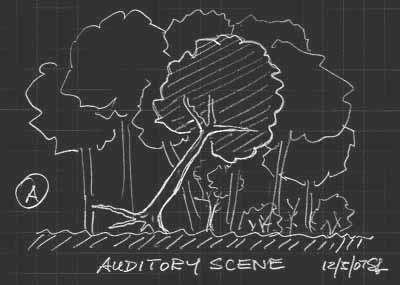
\includegraphics[width=6cm]{./img/tree.jpg}
  \end{center}
\end{frame}

\begin{frame}
  \begin{center}
    \vspace{.2cm}
    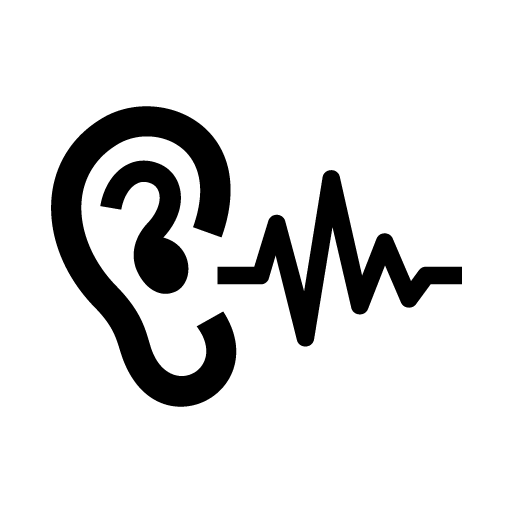
\includegraphics[width=6cm]{./img/listen.png}
  \end{center}
\end{frame}

\begin{frame}
  \begin{center}
    \vspace{.2cm}
    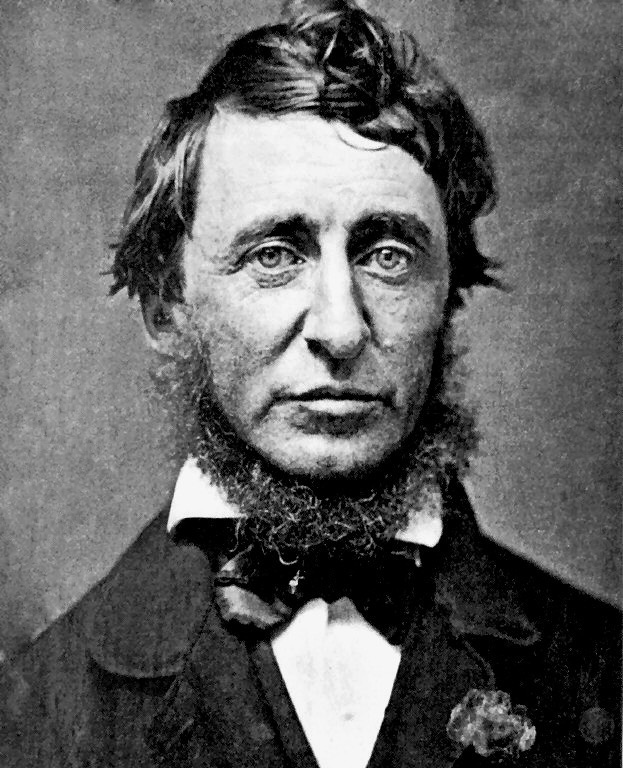
\includegraphics[width=4cm]{./img/thoreau.jpg}
  \end{center}
\end{frame}

\begin{frame}
  \begin{quote}
    Validity then is fundamentally a matter of making the subjectivity of the artist visible in the research design. The need for creating a multi-layered understanding of subject-positions does come out clearly in studies of collaborative creativity.
  \end{quote}
  \begin{flushright}
    \small{- Frisk \& Östersjö, \emph{Beyond Validity}, STM 2013}
  \end{flushright}
\end{frame}

\begin{frame}
  \begin{center}
    \vspace{.2cm}
    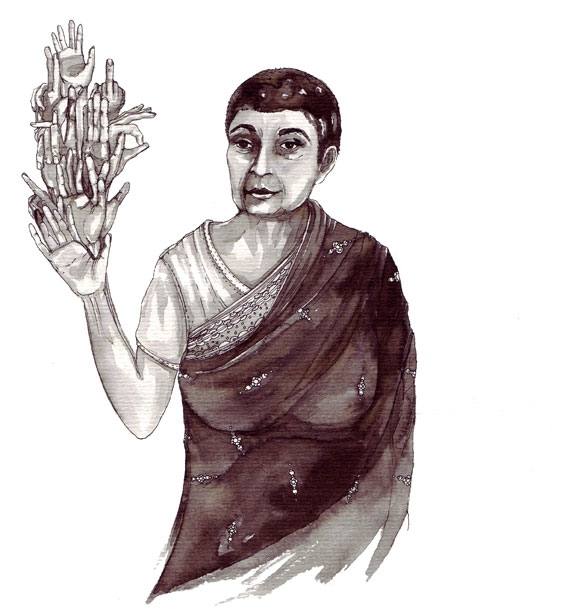
\includegraphics[width=5cm]{./img/spivak.jpg}
  \end{center}
\end{frame}

\begin{frame}
  \begin{center}
    {\huge \color{white} Eye over I}
  \end{center}
\end{frame}

\begin{frame}
  \begin{center}
    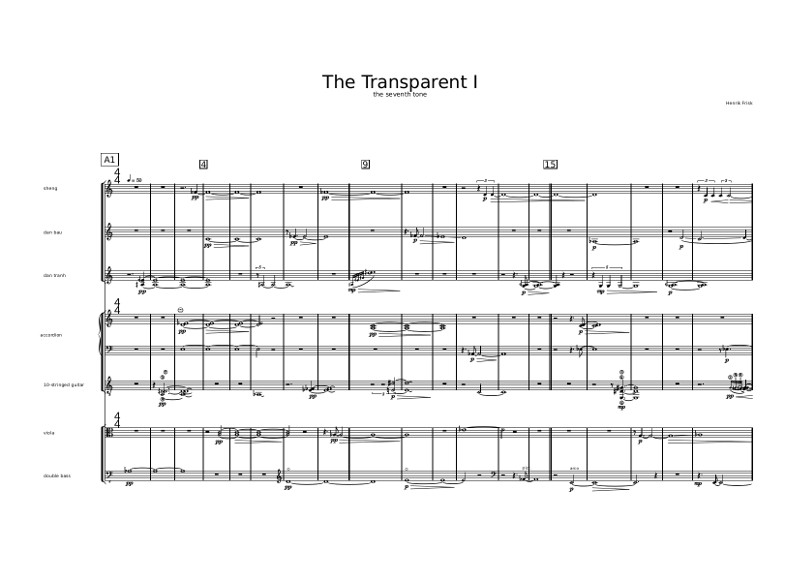
\includegraphics[width=9cm]{./img/transparent.jpg}
  \end{center}
\end{frame}

\begin{frame}
  \begin{center}
    {\huge \color{white} Drinking, and working with text}
  \end{center}
\end{frame}

\begin{frame}
  \begin{center}
    Where is the center?

    \vspace{.2cm}
    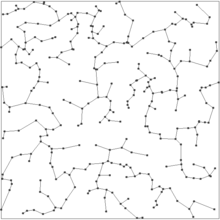
\includegraphics[width=4cm]{./img/center.png}
  \end{center}
\end{frame}

\begin{frame}
  \begin{center}
    \emph{Il n'y a pas de hors-texte}
  \end{center}
\end{frame}

\begin{frame}

  \begin{center}
    \color{white} A Drinking Song (William Butler Yeats)
  \end{center}

    \begin{verse}
      \begin{center}
        Wine comes in at the mouth\\
        And love comes in at the eye;\\
        That’s all we shall know for truth\\
        Before we grow old and die.\\
        I lift the glass to my mouth,\\
        I look at you, and I sigh.
      \end{center}
    \end{verse}
\end{frame}

\begin{frame}
  \begin{center}
    \vspace{.2cm}
    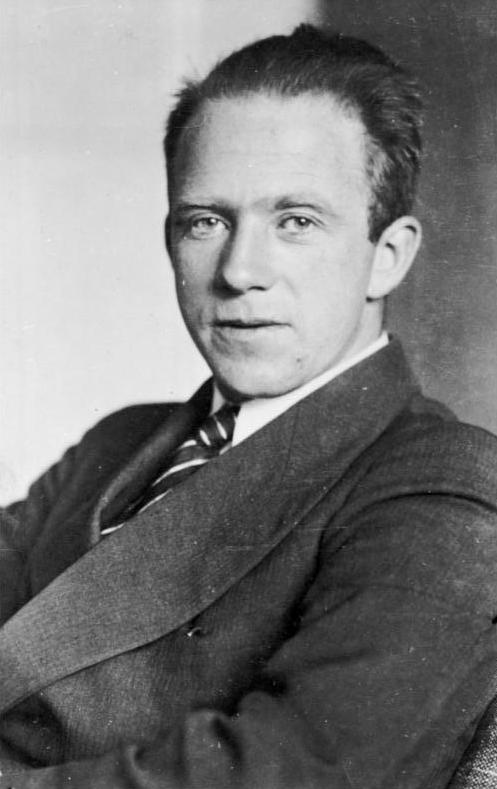
\includegraphics[width=4cm]{./img/heisenberg.jpg}
  \end{center}
\end{frame}

\begin{frame}
  \begin{center}
    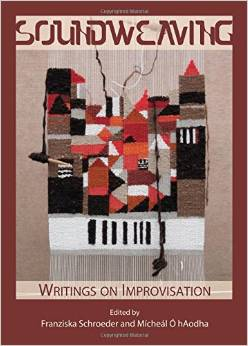
\includegraphics[width=3cm]{./img/soundweaving.jpg}
  \end{center}
\end{frame}

\begin{frame}
  \begin{center}
    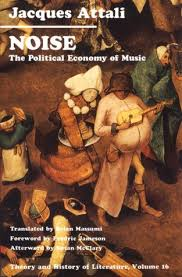
\includegraphics[width=3cm]{./img/noise.jpg}
  \end{center}
\end{frame}

\end{document} 